% ========================================================
% TRABAJO EN GITHUB
% ========================================================
\section{Trabajo en GitHub}\label{sec:github}

El proyecto se aloja en el repositorio público \url{https://github.com/R0SEWT/concurrente}. El
Trabajo Parcial ocupa el directorio \texttt{tp/}, con su propio toolchain y una integración continua
en GitHub Actions que, en cada \emph{pull request}, corre \texttt{go test -race}, \texttt{go vet} y
\texttt{gofmt} sobre el módulo de Go, \texttt{ruff} y \texttt{pytest} sobre el pipeline de datos, y la
regresión de Spin de la Sección~\ref{sec:verificacion} sobre el modelo Promela. La
Figura~\ref{fig:ejec-ci} es el resultado de esos controles sobre la \emph{pull request} que cierra
este entregable.

\begin{figure}[H]
\caption{Controles de integración continua sobre la \emph{pull request} \#50}\label{fig:ejec-ci}
\centering
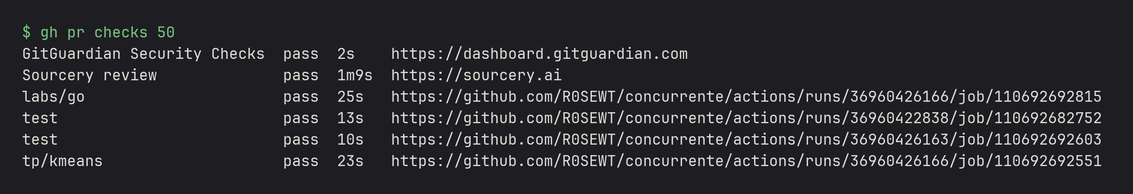
\includegraphics[width=\textwidth]{img/ejec-ci.png}
\end{figure}

\subsection{Flujo Git Flow}

El trabajo sigue Git Flow (Tabla~\ref{tab:ramas}): ningún cambio entra directamente a
\texttt{develop} ni a \texttt{main}, sino por \emph{pull request} desde una rama propia. La
Tabla~\ref{tab:prs} lista los \emph{pull requests} del Trabajo Parcial hasta la fecha de este
informe.

\begin{table}[H]
\caption{Ramas del flujo de trabajo}\label{tab:ramas}
\small
\begin{tabularx}{\textwidth}{@{}L{3.6cm}Y@{}}
\toprule
\textbf{Rama} & \textbf{Uso} \\
\midrule
\texttt{main} & Versión entregada; recibe una fusión por entregable, con un tag (\texttt{pc1},
  \texttt{pc2}, \texttt{tp}) \\
\texttt{develop} & Integración; todo cambio llega por pull request revisado \\
\texttt{feature/*}, \texttt{feat/*} & Una rama por unidad de trabajo, que sale de \texttt{develop} y
  vuelve a ella \\
\texttt{release/*} & Sale de \texttt{develop} para llevar un entregable a \texttt{main}; desde la PC2 el
  release no se hace con \texttt{develop} como rama de origen, porque el repositorio borra la rama
  de origen al fusionar \\
\texttt{hotfix/*} & Arreglo urgente sobre \texttt{main}, que luego se lleva a \texttt{develop} \\
\bottomrule
\end{tabularx}
\end{table}

{\small
\begin{xltabular}{\textwidth}{@{}lL{3.6cm}YL{2.1cm}@{}}
\caption{Pull requests del Trabajo Parcial}\label{tab:prs}\\
\toprule
\textbf{N.º} & \textbf{Autor} & \textbf{Contenido} & \textbf{Estado} \\
\midrule
\endfirsthead
\toprule
\textbf{N.º} & \textbf{Autor} & \textbf{Contenido} & \textbf{Estado} \\
\midrule
\endhead
\bottomrule
\endfoot
\multicolumn{4}{@{}l}{\textit{Entregable 1}} \\
\#3 & \nombreDayana & Propuesta de caso: SENAMHI y ODS 13 & Cerrada \\
\#4 & \nombreDayana & Propuesta de caso: NYC TLC y ODS 11 & Fusionada \\
\#6 & \nombreRody & Limpieza del dataset & Fusionada \\
\#7 & \nombreDayana & Análisis exploratorio (notebook) & Fusionada \\
\#8 & \nombreRody & Bibliografía en BibTeX & Fusionada \\
\#16 & \nombreRody & Informe de PC1 en LaTeX & Fusionada \\
\#17 & \nombreRody & Tabla de commits del informe de PC1 & Fusionada \\
\#18 & \nombreRody & Release PC1: \texttt{develop} $\to$ \texttt{main}, tag \texttt{pc1} & Fusionada \\
\addlinespace
\multicolumn{4}{@{}l}{\textit{Entregable 2}} \\
\#9 & \nombreRody & CI: notebooks sin salidas & Fusionada \\
\#19, \#20 & \nombreRody & Hotfix: compilación de los labs de Go en CI & Fusionadas \\
\#21 & \nombreRody & K-means secuencial y concurrente en Go, Promela y benchmark & Fusionada \\
\#22 & \nombreRody & Informe de PC2 en LaTeX & Fusionada \\
\#32 & \nombreRody & Informe: corrección de las plataformas medidas & Fusionada \\
\#34 & \nombreTercero & Tests de casos borde del K-means concurrente & Fusionada \\
\#35 & \nombreDayana & Documentación del modelo Promela en el informe & Fusionada \\
\#36, \#38 & \nombreRody & Participación en el informe; autómata y contraejemplo de Spin & Fusionadas \\
\#37 & \nombreTercero & Reporte de participación de la PC2 y enlace a los datos & Fusionada \\
\#39 & \nombreRody & Empaquetado de la entrega & Fusionada \\
\#40--\#42 & \nombreRody & Release PC2: \texttt{develop} $\to$ \texttt{main}, tag \texttt{pc2} & Fusionadas \\
\addlinespace
\multicolumn{4}{@{}l}{\textit{Entregable 3}} \\
\#43 & \nombreRody & Spin: deadlock, exclusión mutua y progreso con LTL y mutantes & Fusionada \\
\#44 & \nombreRody & Informe del TP en LaTeX, a partir del de la PC2 & Fusionada \\
\#45 & \nombreRody & GAPs con IA, participación, empaquetado y guion del video & Fusionada \\
\#46 & \nombreRody & Historial: alias de autor unificado por nombre & Fusionada \\
\#48 & \nombreTercero & Conclusiones y recomendaciones individuales & Fusionada \\
\#49 & \nombreDayana & Conclusiones individuales y compilación del informe en macOS & Fusionada \\
\#50 & \nombreRody & Visor rediseñado, capturas regenerables y PRs del grupo en el informe & Fusionada \\
\end{xltabular}
}

\subsection{Historial de commits por integrante}

Las Tablas~\ref{tab:commits-autor} y~\ref{tab:commits} se generan desde el repositorio con
\texttt{./generar-historial.sh}. La tabla por integrante separa lo entregado en cada entregable, con
los tags \texttt{pc1} y \texttt{pc2} como cortes, y el listado de commits del Entregable 3 indica
cuáles ya forman parte de \texttt{main} al generar la tabla.

% Generado por generar-historial.sh el 2026-09-29. No editar a mano.
\begin{table}[H]
\caption{Commits del Trabajo Parcial por integrante y entregable}\label{tab:commits-autor}
\footnotesize
\begin{tabular}{@{}lrrrr@{}}
\toprule
\textbf{Integrante} & \textbf{PC1} & \textbf{PC2} & \textbf{TP (nuevos)} & \textbf{Merges de PR (TP)} \\
\midrule
Dayana Kety Gómez Rodriguez & 5 & 3 & 0 & 0 \\
Julio Cesar Meza Alfaro & 0 & 4 & 0 & 0 \\
R0SEWT-CGIAR & 0 & 1 & 0 & 0 \\
Rody Sebastian Vilchez Marin & 21 & 29 & 1 & 2 \\
\bottomrule
\end{tabular}

{\footnotesize\textit{Nota.} Commits que tocan \texttt{tp/} o \texttt{docs/}. PC1 cuenta hasta el tag \texttt{pc1} (entregado el 13 de septiembre); PC2, de \texttt{pc1} al tag \texttt{pc2} (entregado el 27 de septiembre); TP, lo que no está en \texttt{pc2}, en todas las ramas publicadas en \texttt{origin}. Los merges de PR se cuentan aparte porque no tocan archivos por sí mismos.\par}
\end{table}

{\small
\begin{xltabular}{\textwidth}{@{}L{1.9cm}L{2.7cm}L{1.4cm}Yc@{}}
\caption{Commits del Entregable 3, del más reciente al más antiguo}\label{tab:commits}\\
\toprule
\textbf{Fecha} & \textbf{Autor} & \textbf{Commit} & \textbf{Mensaje} & \textbf{En \texttt{main}} \\
\midrule
\endfirsthead
\toprule
\textbf{Fecha} & \textbf{Autor} & \textbf{Commit} & \textbf{Mensaje} & \textbf{En \texttt{main}} \\
\midrule
\endhead
\bottomrule
\endfoot
2026-09-28 & Rody Sebastian Vilchez Marin & \texttt{a86af92} & Verificar con LTL la exclusión mutua y el progreso, con un mutante por propiedad & no \\
\end{xltabular}
}

{\footnotesize\textit{Nota.} «En \texttt{main}» indica si el commit ya forma parte de \texttt{origin/main} al generar esta tabla; los que dicen «no» están en una rama publicada pendiente de fusión.\par}


\subsection{Participación de los integrantes}

Cada integrante tiene al menos una \emph{pull request} propia en este entregable; los commits de cada
uno están en las Tablas~\ref{tab:commits-autor} y~\ref{tab:commits}.

\paragraph{\nombreRody{} (coordinador).} Extendió el modelo Promela con las fórmulas LTL de
exclusión mutua y de progreso, los mutantes de deadlock y de barrera omitida, y la regresión de siete
casos que corre en la integración continua (PR~\#43); armó este informe a partir del de la PC2 con
la Sección~\ref{sec:verificacion} (PR~\#44); hizo el análisis de GAPs con IA y su contraste contra
el código, el guion del video y el empaquetado de la entrega (PR~\#45); resolvió la interpretación de
los clusters con agregación espaciotemporal hacia el ODS~11 y desarrolló la aplicación de
exploración interactiva (Sección~\ref{sec:interpretacion-clusters}). Revisó e integró las \emph{pull requests} del resto del grupo.

\paragraph{\nombreDayana.} Contrastó la implementación en Go con el modelo Promela (\emph{worker
pool}, acumuladores privados y barrera) y redactó sus conclusiones y recomendaciones sobre esa
correspondencia; además adaptó \texttt{compilar.sh} para que el informe compile en macOS con MacTeX
y conserve el historial anterior si no puede regenerarlo, y excluyó del repositorio los artefactos
de LaTeX (PR~\#49).

\paragraph{\nombreTercero.} A partir de los tests de casos borde que aportó en la PC2 (más
\emph{workers} que puntos y clusters vacíos), redactó sus conclusiones sobre por qué la corrección de
una ejecución no sustituye a la verificación de todos los entrelazados, y sobre el costo de
coordinación que el speedup deja ver con pocos datos (PR~\#48).
